\thispagestyle{empty}
\vspace*{\fill}
\addcontentsline{toc}{section}{Fun Zone}
\begin{center}
    \section*{\normalfont\rmfamily\cursive\fontsize{60}{72}\selectfont Fun Zone}
\end{center}
\vspace*{\fill}

\newpage

\begin{center}
  {\LARGE\bfseries\rmfamily\color{IEEEblue} Electronics Crossword\par}
  \vspace{0.2em}
  {\small\itshape Test your knowledge of circuits, logic and electronic devices.\par}
  \vspace{0.6em}
  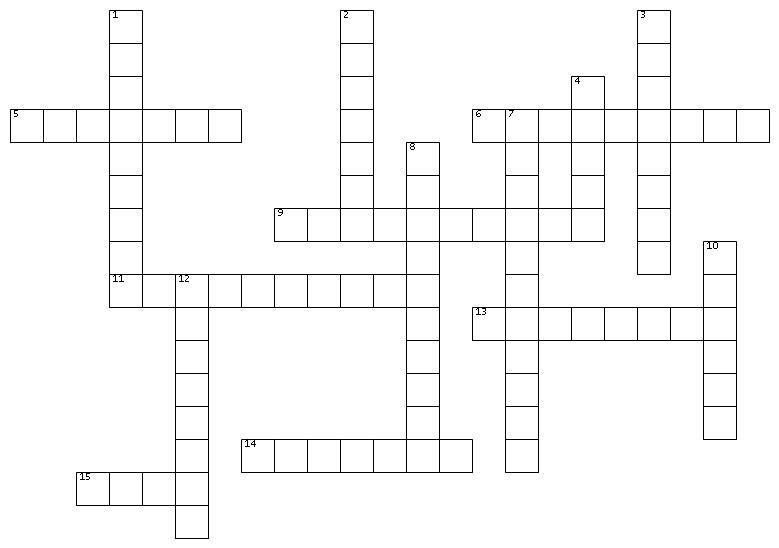
\includegraphics[width=0.94\textwidth]{assets/images/ecrossword.png}
\end{center}

\vspace{0.5em}
\noindent
\begin{minipage}[t]{0.485\textwidth}
  {\large\bfseries\rmfamily\color{IEEEblue} ACROSS}\par
  \vspace{0.2em}
  {\color{IEEEorange}\rule{\linewidth}{1pt}}\par
  \smallskip
  \footnotesize
  \begin{enumerate}[leftmargin=2.1em,itemsep=3pt,topsep=0pt,parsep=0pt]
    \item[\textbf{5.}] Voltage reference circuit that provides a stable output independent of temperature
    \item[\textbf{6.}] Total opposition a circuit offers to alternating current at a given frequency
    \item[\textbf{9.}] Passive device used to reduce the power of a signal without distorting its waveform
    \item[\textbf{11.}] Lagging of an effect behind its cause seen in Schmitt triggers
    \item[\textbf{13.}] Bistable multivibrator used as a basic memory element to store one bit
    \item[\textbf{14.}] Combinational circuit that converts multiple input lines into a coded binary output
    \item[\textbf{15.}] Term for a circuit node that absorbs current coming from a load
  \end{enumerate}
\end{minipage}%
\hfill
\begin{minipage}[t]{0.485\textwidth}
  {\large\bfseries\rmfamily\color{IEEEblue} DOWN}\par
  \vspace{0.2em}
  {\color{IEEEorange}\rule{\linewidth}{1pt}}\par
  \smallskip
  \footnotesize
  \begin{enumerate}[leftmargin=2.1em,itemsep=3pt,topsep=0pt,parsep=0pt]
    \item[\textbf{1.}] Difference between the upper and lower frequencies in a continuous band of signals
    \item[\textbf{2.}] Trigger circuit that uses positive feedback to clean up noisy input signals
    \item[\textbf{3.}] Voltage-variable capacitor diode used in RF tuning circuits
    \item[\textbf{4.}] Special diode designed to reliably allow current to flow backwards when a specific reverse voltage is reached
    \item[\textbf{7.}] Combinational logic circuit that selects one of several input signals and forwards it to a single line
    \item[\textbf{8.}] Multivibrator circuit that produces a single output pulse when triggered
    \item[\textbf{10.}] Small unwanted residual AC voltage remaining after rectification
    \item[\textbf{12.}] Fast-switching diode featuring a low forward voltage drop
  \end{enumerate}
\end{minipage}

\newpage

\begin{center}
  {\LARGE\bfseries\rmfamily\color{IEEEblue} Circuit Seekers\par}
  \vspace{0.15em}
  {\large\bfseries\rmfamily Electronics Word Search\par}
  \vspace{0.2em}
  {\small\itshape Find the hidden terms from electronics, communication and semiconductor engineering.\par}

  \vspace{1em}
  
\includegraphics[width=0.9\textwidth]{assets/images/ewordsearch.png}

  \vspace{1em}
  {\large\bfseries\rmfamily\color{IEEEblue} WORD BANK}\par
  \vspace{0.2em}
  {\color{IEEEorange}\rule{0.94\textwidth}{1pt}}\par
  \vspace{0.6em}

  \footnotesize\rmfamily
  \setlength{\tabcolsep}{8pt}
  \renewcommand{\arraystretch}{1.35}
  \begin{tabular}{@{}llll@{}}
    MICROPROCESSOR & DRAIN         & MODULATION     & AMMETER \\
    FREQUENCY      & SOURCE        & MULTIVIBRATOR  & CONDUCTOR \\
    CAPACITANCE    & ANODE         & FLIPFLOP       & INSULATOR \\
    INDUCTANCE     & CATHODE       & ENCODER        & SEMICONDUCTOR \\
    CONDUCTIVITY   & AMPLIFIER     & DECODER        & PHOTODIODE \\
    SILICON        & OSCILLATOR    & COMPARATOR     & TRANSDUCTOR \\
    GATE           & WAVEFORM      & REGULATOR      & TRANSMISSION \\
    HARMONICS      & ATTENUATION   & VOLTMETER      & SENSITIVITY \\
    RADIATION      & POLARIZATION  & GAIN           & RECTIFICATION \\
    TRANSCEIVER    & DEMODULATOR   & THERMISTOR     & VARISTOR
  \end{tabular}
\end{center}

\newpage

\begin{center}
  {\LARGE\bfseries\rmfamily\color{IEEEblue} Circuit Brain Teasers\par}
  \vspace{0.2em}
  {\small\itshape Who am I? Identify each electronic device, concept or architecture.\par}
\end{center}

\vspace{0.7em}
\begin{tcolorbox}[
  colback=black!2,
  colframe=IEEEblue!75!black,
  boxrule=0.6pt,
  arc=0mm,
  left=5mm,
  right=5mm,
  top=4mm,
  bottom=4mm
]
  \small
  \begin{enumerate}[leftmargin=2.1em,itemsep=0.75em,topsep=0pt,parsep=0pt]
    \item I am a specialized antenna whose physical geometry contains radio frequency switches. By turning those switches on or off, I can instantly alter my operating frequency, radiation pattern, or polarization on the fly. Who am I?

    \item I contain an ALU, control unit, and registers on a single integrated circuit, serving as the central engine that fetches, decodes, and executes instructions line by line. Who am I?

    \item I consist of multiple individual radiating elements fed with specific phase delays, allowing me to steer a narrow electromagnetic beam electronically without moving a single part. Who am I?

    \item I sit right next to the processor core, operating at near-CPU speeds. I store copies of frequently accessed RAM data so the execution unit never starves waiting for memory access. Who am I?

    \item I stack multiple antenna elements together using specialized spatial arrangements to drastically increase channel capacity and link reliability over an ultra-wide frequency spectrum. Who am I?

    \item I am an architecture technique where multiple instruction steps---fetch, decode, execute, writeback---are overlapped in parallel stages, drastically boosting clock-cycle efficiency. Who am I?

    \item I am a microstrip planar antenna featuring a flat metal patch printed on top of a dielectric substrate above a ground plane, widely used for compact wireless applications. Who am I?

    \item I am a physical pin on a microprocessor. When a peripheral pulls my voltage line, I force the CPU to immediately suspend its current code execution and run a specialized handler routine. Who am I?

    \item I am a ratio that measures how efficiently radio frequency power is transmitted from a feedline into an antenna, reaching an ideal value of 1:1 when there are no reflected standing waves. Who am I?

    \item I am a specialized register inside a microprocessor that holds the memory address of the very next instruction waiting to be fetched and executed. Who am I?
  \end{enumerate}
\end{tcolorbox}

\vfill
\begin{center}
  {\small\bfseries\rmfamily\color{IEEEblue}
  Answers to the Fun Zone puzzles are given on the next page.\par}
\end{center}
